\documentclass[titlepage=firstiscover, captions=tableheading, bibliography=totoc]{scrartcl}
\usepackage[autostyle=true,german=quotes]{csquotes}
\usepackage{scrhack}
\usepackage{enumitem}
\usepackage{caption}
\usepackage[aux]{rerunfilecheck}
\usepackage{subcaption}
\usepackage{fontspec}
\usepackage[dvips]{graphicx}
\usepackage{floatflt,epsfig}

\usepackage{polyglossia}
\setmainlanguage{german}

\usepackage[unicode]{hyperref}
\usepackage{bookmark}
\title{Computational Physics}
\subtitle{Übungsblatt 7}
\author{
Miriam Simm\\
\texorpdfstring{\href{mailto:miriam.simm@tu-dortmund.de}{miriam.simm@tu-dortmund.de}\and}{,}
Katrin Bolsmann\\
\texorpdfstring{\href{mailto:katrin.bolsmann@tu-dortmund.de}{katrin.bolsmann@tu-dortmund.de}}{,}\\
\\
Mario Alex Hollberg\\
\texorpdfstring{\href{mailto:mario-alex.hollberg@tu-dortmund.de}{mario-alex.hollberg@tu-dortmund.de}}{}
}
\date{Abgabe: 15. Mai 2020}
\usepackage{amsmath}
\usepackage{amssymb}
\usepackage{mathtools}
\usepackage[
    math-style=ISO,
    bold-style=ISO,
    sans-style=italic,
    nabla=upright,
    partial=upright,
]{unicode-math}

\setmathfont{Latin Modern Math}

\usepackage[
  locale=DE,
  separate-uncertainty=true,
  per-mode=symbol-or-fraction,
]{siunitx}

\usepackage{multicol}
\setlength{\columnsep}{1pt} %space between columns

\usepackage{booktabs}
\usepackage[x11names, table]{xcolor}
\usepackage{graphicx}
\usepackage{grffile}
\usepackage{xfrac}
\usepackage{xcolor}

\usepackage{float}
\floatplacement{figure}{h}
\floatplacement{table}{h}
\usepackage[
  section,
  below,
]{placeins}

\usepackage{expl3}
\usepackage{xparse}
\ExplSyntaxOn
\NewDocumentCommand \E {} {\symup{e}}
\ExplSyntaxOff

% Literaturverzeichnis
\usepackage[
  backend=biber,
]{biblatex}
% Quellendatenbank
\addbibresource{literatur.bib}

\usepackage[
  version=4,
  math-greek=default,
  text-greek=default,
]{mhchem}


\raggedcolumns


\begin{document}

\maketitle

\section*{Simulation des zweidimensionalen Ising-Modells}
In dieser Aufgabe mit dem Metropolis-Algorithmus als Monte-Carlo-Methode ein Ising-Modell in zwei Dimensionen 
ohne externes Magnetfeld simuliert. Das Modell hat die Energie
\begin{equation*}
    \mathcal{H} = - \sum_{i, j \, \text{n.N.}} \sigma_i \sigma_j \, ,
\end{equation*}
wobei nur über nächste Nachbarn summiert wird. Es wird ein zweidimensionales System der Größe $A = L \times L$
mit periodischen Randbedingungen, die in der Funktion \texttt{randbedingungen} implementiert sind, betrachtet. 
Hier verwendet wird ein System der Größe $100 \times 100$ mit entsprechend 10000 Teilchen.

\subsubsection*{Initialisierung}
Vor Beginn der Messung erfolgt eine Initialisierung. Die Teilchen werden dazu den Gitterplätzen zugeordnet, was 
in der Funktion \texttt{initialisierung} implementiert ist. Die Teilchen werden in einer $3 \times N$-Matrix gespeichert, 
wobei die ersten beiden Zeilen jeweils die $x$- und $y$-Koordinate und die dritte Zeile die Spinausrichtung 
angibt. Die Spins können zu Beginn entweder vollständig geordnet sein, oder eine zufällige Ausrichtung haben,
was über den Übergabewert \texttt{ordnung} gesteuert wird. 

\subsubsection*{Äquilibrierung}
Dem System werden mit dem Metropolis-Algorithmus Spin-Flips angeboten, was in der Funktion \texttt{aequilibrierung}
und \texttt{metropolis}
implementiert ist. Nach einer Äquilibrierungsphase mit $10^5$ Schritten werden für die drei Temperaturen $k_\text{B}T = 1.5$,
$k_\text{B}T = 2.27$ und $k_\text{B}T = 3$ Momentaufnahmen erstellt, die in Abbildung \ref{fig:2_moment_1}, \ref{fig:2_moment_2} 
und \ref{fig:2_moment_3} dargestellt sind.
\FloatBarrier
\begin{figure}[H]
    \centering
    \includegraphics[width=0.8\textwidth]{momentaufnahme_1.pdf}
    \caption{Momentaufnahme des Systems bei $k_\text{B}T = 1.5$.}
    \label{fig:2_moment_1}
\end{figure}
\FloatBarrier
\noindent
\FloatBarrier
\begin{figure}[H]
    \centering
    \includegraphics[width=0.8\textwidth]{momentaufnahme_2.pdf}
    \caption{Momentaufnahme des Systems bei $k_\text{B}T \approx 2.27$.}
    \label{fig:2_moment_2}
\end{figure}
\FloatBarrier
\noindent
\FloatBarrier
\begin{figure}[H]
    \centering
    \includegraphics[width=0.8\textwidth]{momentaufnahme_3.pdf}
    \caption{Momentaufnahme des Systems bei $k_\text{B}T = 3$.}
    \label{fig:2_moment_3}
\end{figure}
\FloatBarrier
\noindent
In Abbildung \ref{fig:2_moment_1} ist deutlich die spontane ferromagnetische Ordnung sichtbar, die sich bei $T < T_c$
ausbildet, da nahezu alle Spins in eine Richtung zeigen.
Abbildung \ref{fig:2_moment_2} zeigt, dass sich im Bereich der kritischen Temperatur $T_c$ Bereiche ausbilden, 
in denen die Spins entweder nach oben oder nach unten zeigen. Bei höherer Temperatur $T > T_c$ wird das System
aufgrund thermischer Fluktuationen ungeordnet, wie in Abbildung \ref{fig:2_moment_3} ersichtlich ist. 

Anschließend wird in der Äquilibrierungsphase die mittlere Energie pro Spin als Funktion der Simulationszeit gemessen
\begin{equation*}
    e(t) = \frac{E(t)}{N} = \frac{\langle \mathcal{H} \rangle}{N} \, .
\end{equation*} 
Die Ergebnisse für geordnete Anfangsbedingungen sind in Abbildung \ref{fig:2_energie_geordnet} dargestellt.
\FloatBarrier
\begin{figure}[H]
    \centering
    \includegraphics[width=0.8\textwidth]{Energie_Equi_geordnet.pdf}
    \caption{Mittlere Energie pro Spin als Funktion der Simulationszeit $t$ in der Äquilibrierungsphase mit geordneter Spinausrichtung als Anfangsbedingung.}
    \label{fig:2_energie_geordnet}
\end{figure}
\FloatBarrier
\noindent
Dasselbe wird zusätzlich für völlig ungeordnete Spins als Anfangsbedingung durchgeführt. Die Ergebnisse sind 
in Abbildung \ref{fig:2_energie_1_ungeordnet} dargestellt.
\FloatBarrier
\begin{figure}[H]
    \centering
    \includegraphics[width=0.8\textwidth]{Energie_Equi.pdf}
    \caption{Mittlere Energie pro Spin als Funktion der Simulationszeit $t$ in der Äquilibrierungsphase mit zufälliger Spinausrichtung als Anfangsbedingung.}
    \label{fig:2_energie_ungeordnet}
\end{figure}
\FloatBarrier
\noindent
Die Anfangsbedingungen beeinflussen die Simulation offenbar stark. Unabhängig von den Anfangsbedingungen 
äquilibriert das System, sobald es einen annähernd konstanten Wert erreicht, also nach etwa 4-5 Zeitschritten bei zufälliger 
Ausrichtung der Spins als Anfangsbedingung und etwa 3 Zeitschritten bei geordneten Anfangsbedigungen, jedoch mehr für $k_\text{B}T = 3$.
Da bei dieser Simulation die Äquilibrierungszeit etwas zu kurz gewählt wurde, wie in den Abbildungen auch ersichtlich ist,
sind diese Ergebnisse noch einmal im Anhang \ref{sec:anhang} aus einer Simulation mit 6400 Teilchen dargestellt.

\subsubsection*{Messung}
Nun wird die Zeit nach der Äquilibrierungsphase betrachtet, wobei als Anfangsbedingung eine zufällige Spinausrichtung
gewählt wird. Die Messung erfolgt nun nach jedem Sweep. 
Pro Sweep wird jedem Spin im Mittel einmal ein Spinflip angeboten. Gemessen wird die Magnetisierung
\begin{equation*}
    \langle m \rangle = \left\langle \frac{1}{N} \sum_i \sigma_i\right\rangle \, ,
\end{equation*}
und der Betrag der Magnetisierung
\begin{equation*}
    \langle | m | \rangle = \left\langle \frac{1}{N} \left| \sum_i \sigma_i \right| \right\rangle \, ,
\end{equation*}
pro Spin sowie die Energie für die gleichen Temperaturen wird bei der in den vorherigen Messungen. Die Ergebnisse sind in Abbildung 
\ref{fig:energie}, \ref{fig:magnetisierung} und \ref{fig:betrag_magnetisierung} dargestellt.
\FloatBarrier
\begin{figure}[H]
    \centering
    \includegraphics[width=0.8\textwidth]{Energie.pdf}
    \caption{Mittlere Energie pro Spin als Funktion der Simulationszeit $t$.}
    \label{fig:energie}
\end{figure}
\FloatBarrier
\noindent
\FloatBarrier
\begin{figure}[H]
    \centering
    \includegraphics[width=0.8\textwidth]{Magnetisierung.pdf}
    \caption{Magnetisierung pro Spin als Funktion der Simulationszeit $t$.}
    \label{fig:magnetisierung}
\end{figure}
\FloatBarrier
\noindent
\FloatBarrier
\begin{figure}[H]
    \centering
    \includegraphics[width=0.8\textwidth]{Betrag_Magnetisierung.pdf}
    \caption{Betrag der Magnetisierung pro Spin als Funktion der Simulationszeit $t$.}
    \label{fig:betrag_magnetisierung}
\end{figure}
\FloatBarrier
\noindent
Alle Messungen sind in der Funktion \texttt{spinflip} implementiert.
In Abbildung \ref{fig:magnetisierung} und \ref{fig:betrag_magnetisierung} ist deutlich der Phasenübergang bei $T = T_c$ sichtbar, 
da die Magnetisierung stark zwischen den Werten für $k_\text{B}T = 1.5$ und $k_\text{B}T = 3$ fluktuiert. 
Außerdem ist erkennbar, dass unterhalb der kritischen Temperatur eine nicht-verschwindende Magentisierung auftritt, 
da sich das System spontan magnetisch ordnet.
Der Verlauf der Energie in Abbildung \ref{fig:energie} zeigt, dass die Energie nach der kurzen Äquilibrierungsphase 
um einen konstanten Wert fluktuiert. 

\section*{Aufgabe 3: Simulated Annealing}
Gegeben seien N 2-dimensionale Ortsvektoren $\vec{r}_i$ und eine initiale Permutation $\pi_0$ der Indizes der Ortsvektoren.
Die geschlossene Weglänge einer Permutation ist gegeben durch
\begin{equation*}
L(\pi) = \sum_{i=2}^N |\vec{r}_{\pi(i)}-\vec{r}_{\pi(i-1)}| + |\vec{r}_{\pi(1)}-\vec{r}_{\pi(N)}|\, .
\end{equation*}
Ziel der Aufgabe ist es jene Permutation zu finden, die die Weglänge minimiert.

\subsection*{1. Implementierung des Algorithmus}
Das Problem, welches in der Vorlesung als \textit{Travelling Salesman Problem} behandelt wurde, wird mit einer Variante des Metropolis Algorithmus gelöst.
\begin{itemize}
\item Halte Anfangs- und Endpunkt fest
\item Starte mit beliebiger Strecke und hoher fiktiver Temperatur $T_\text{start}$
\item Wiederhole S mal: Tausche zwei zufällige Ortsvektoren und berechnet Streckenänderung $\Delta L$
\begin{itemize}
\item[*] $\Delta L \leq 0 \, \rightarrow$ Annahme der Veränderung
\item[*] $\Delta L > 0 \, \rightarrow$ ziehe $P \in (0,\,1)$ und nehme an wenn $P < e^{-\beta\Delta L}$
\end{itemize}
\item Verringere Temperatur um den Dämpfungsfaktor $d\in (0,\, 1)$ bis Endtemperatur $T_\text{end}$ erreicht
\end{itemize}

\subsection*{2. Initialisierung der Startkonfiguration}
Die Ortsvektoren werden wie in Abbildung \ref{fig:3_1} angeordnet.
Diese Reihenfolge entspricht zugleich der des kürzesten Weges.
\FloatBarrier
\begin{figure}[H]
    \centering
    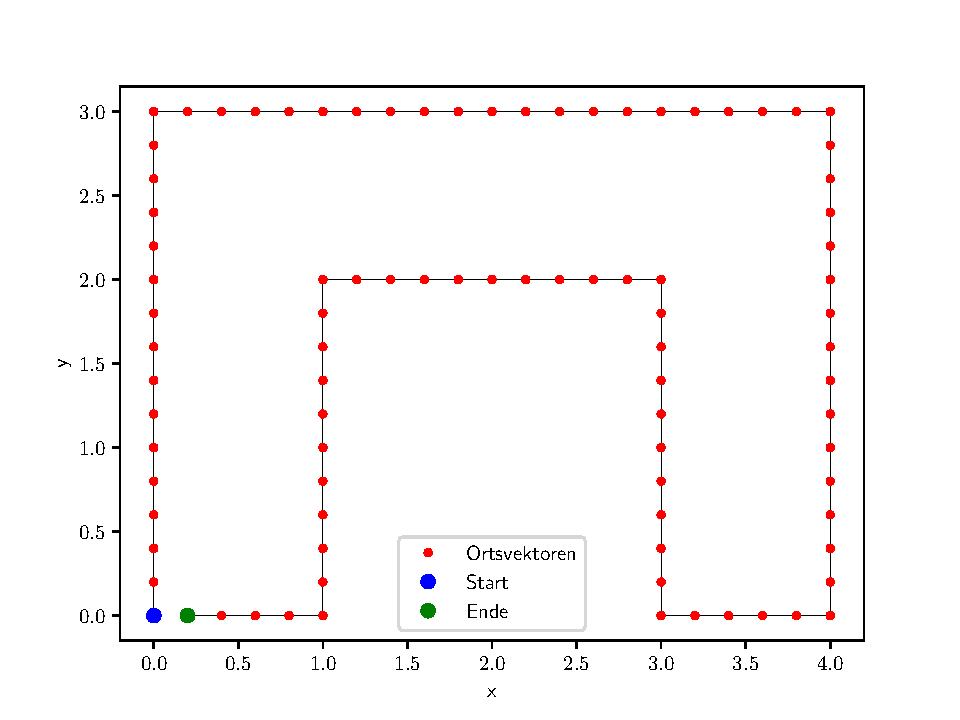
\includegraphics[width=0.8\textwidth]{Initialisierung.pdf}
    \caption{Verteilung der Ortsvektoren mit der kürzesten Strecke von $17$.}
    \label{fig:3_1}
\end{figure}
\FloatBarrier
\noindent

Um die initiale Startpermutation zu erhalten wird der zu \ref{fig:3_1} gehörende Permutationsvektor zufällig angeordnet.
Die erhaltene Startkonfiguration ist in Abbildung \ref{fig:3_2} dargestellt.

\FloatBarrier
\begin{figure}[H]
    \centering
    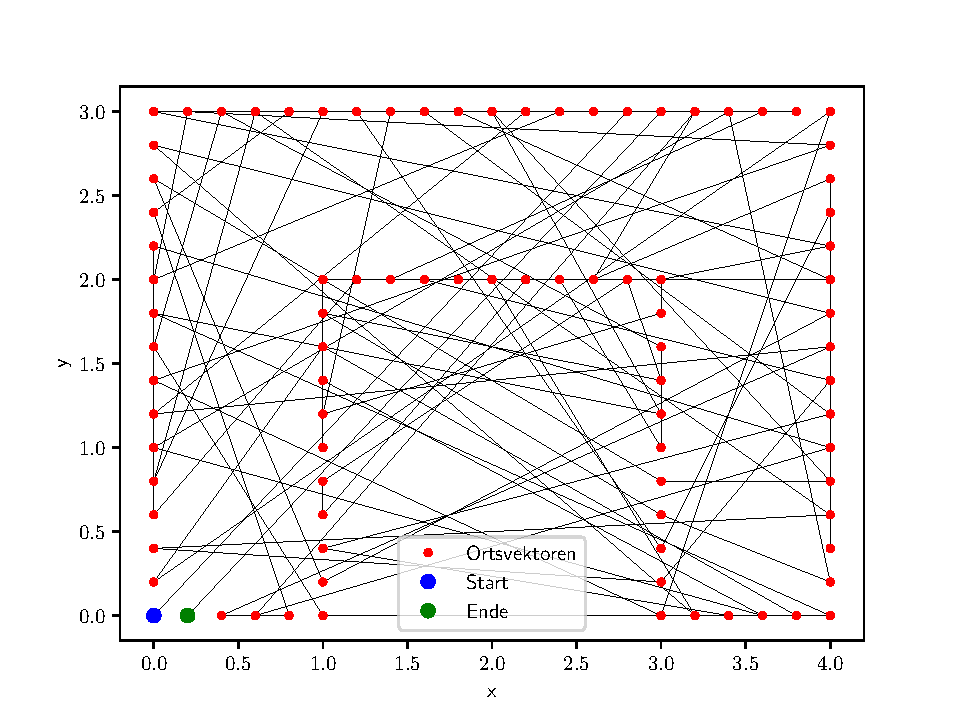
\includegraphics[width=0.8\textwidth]{Startkonfig.pdf}
    \caption{Startkonfiguration, Start- und Endpunkt wurden festgehalten. Diese entsprechen also den gleichen wie in Abbildung \ref{fig:3_2}.
    Die Strecke beträgt hier $208.965$.}
    \label{fig:3_2}
\end{figure}
\FloatBarrier
\noindent

\subsection*{3. Berechnung der optimalen Permutation}
Der Algorithmus sollte für die in $2.$ berechnete Startkonfiguration angewendet werden.
Dazu wurden die Parameter
\begin{align*}
T_\text{start} &= 10 \\
T_\text{end} &= 10^{-2} \\
d &\in \{0.9,\,0.99,\,0.999\} \\
S &\in \{10,\,100,\,1000\,10000\} 
\end{align*}
verwendet.
Die sich ergebenen Strecken sind in den Plots \ref{fig:3_3} \ref{fig:3_4} \ref{fig:3_5} \ref{fig:3_6} zu sehen.
\FloatBarrier
\begin{figure}[H]
    \centering
    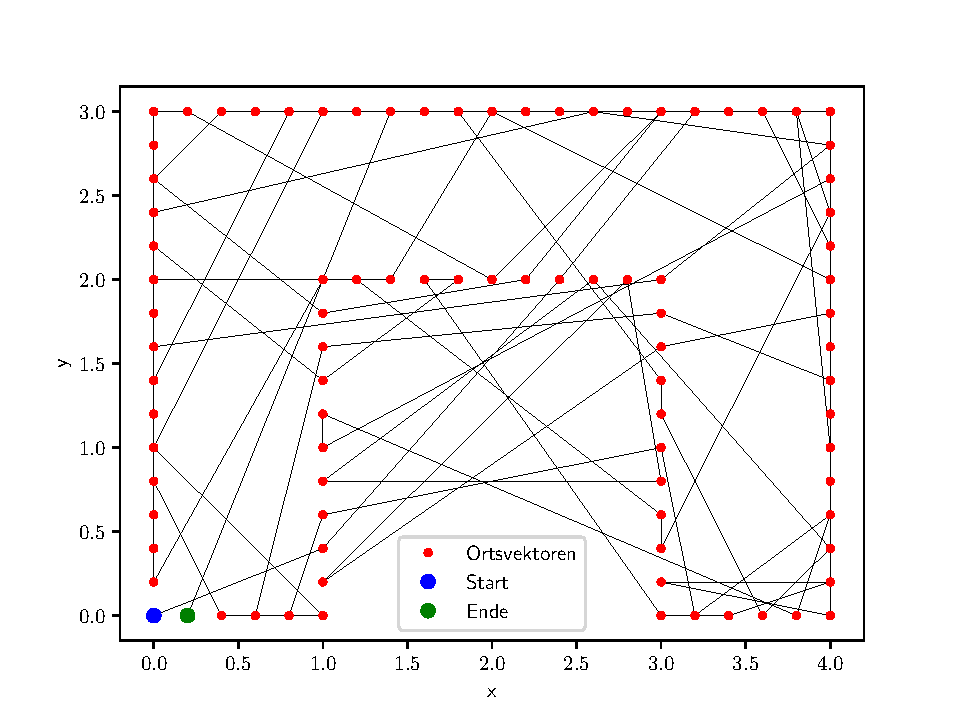
\includegraphics[width=0.8\textwidth]{Strecke_d_0.9_S_10.pdf}
    \caption{Die optimale Strecke welche sich nach der Ausführung des Algorithmus mit $d=0.9$ und $S=10$ ergibt. 
    Die Gesamtstrecke beträgt $106.71$. Sie wurde also im Vergleich zur Startkonfiguration um circa $49\%$ um reduziert.}
    \label{fig:3_3}
\end{figure}
\FloatBarrier
\noindent
\FloatBarrier
\begin{figure}[H]
    \centering
    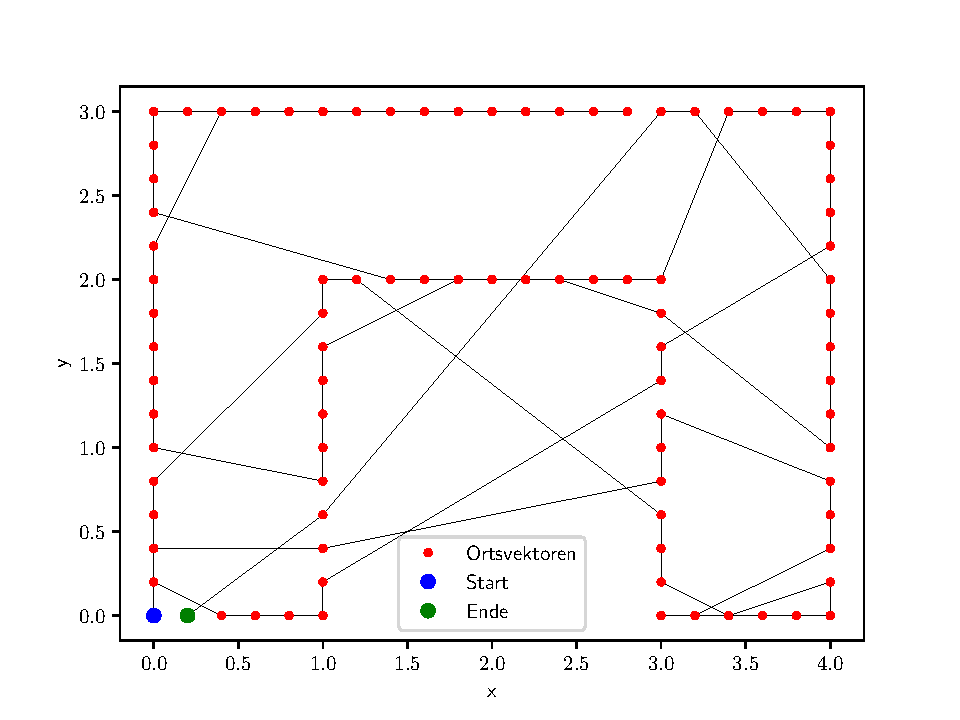
\includegraphics[width=0.8\textwidth]{Strecke_d_0.9_S_1000.pdf}
    \caption{Die optimale Strecke welche sich nach der Ausführung des Algorithmus mit $d=0.9$ und $S=1000$ ergibt. 
    Die Gesamtstrecke beträgt $44.19$. Sie wurde also im Vergleich zur Startkonfiguration um circa $79\%$ um reduziert.}
    \label{fig:3_4}
\end{figure}
\FloatBarrier
\noindent
\FloatBarrier
\begin{figure}[H]
    \centering
    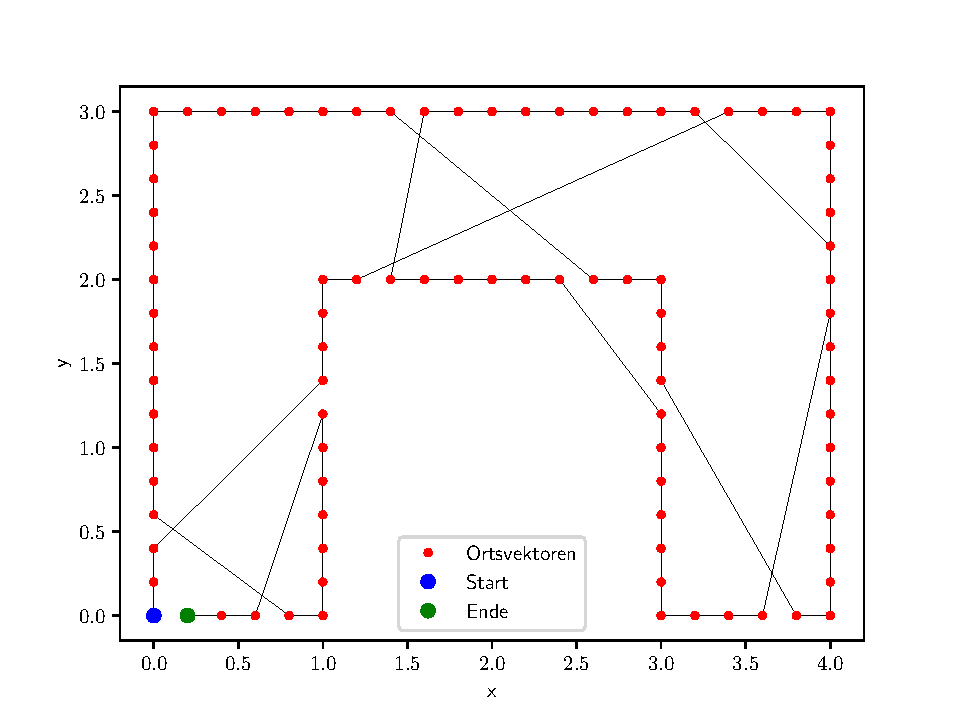
\includegraphics[width=0.8\textwidth]{Strecke_d_0.99_S_1000.pdf}
    \caption{Die optimale Strecke welche sich nach der Ausführung des Algorithmus mit $d=0.99$ und $S=1000$ ergibt. 
    Die Gesamtstrecke beträgt $30.87$. Sie wurde also im Vergleich zur Startkonfiguration um circa $85\%$ um reduziert.}
    \label{fig:3_5}
\end{figure}
\FloatBarrier
\noindent
\FloatBarrier
\begin{figure}[H]
    \centering
    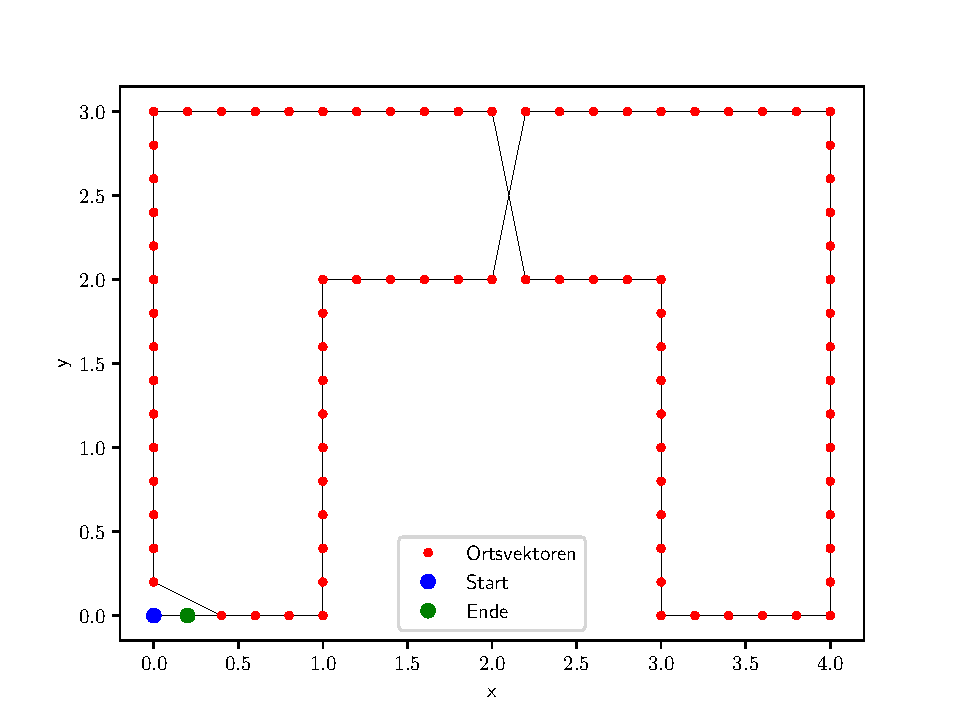
\includegraphics[width=0.8\textwidth]{Strecke_d_0.999_S_10000.pdf}
    \caption{Die optimale Strecke welche sich nach der Ausführung des Algorithmus mit $d=0.999$ und $S=10000$ ergibt. 
    Die Gesamtstrecke beträgt $20.29$. Sie wurde also im Vergleich zur Startkonfiguration um circa $90\%$ um reduziert.}
    \label{fig:3_6}
\end{figure}
\FloatBarrier
\noindent
Bei dem letzten Plot beträgt die Abweichung der minimalen Strecke noch circa $19\%$ von der optimalen Strecke.
Auffällig ist, dass die Strecke sich bereits für geringe Parameter $d=0.9$ $S=10$ stark reduziert.
Jedoch kann für sehr viele Vorschläge $S$ und sehr schwache Dämpfung $d$ immer noch nicht die optimale Strecke erreicht werden.
Das liegt vermutlich daran, dass zu Beginn des Algorithmus die Annahmewahrscheinlichkeit noch sehr hoch ist, während sie gegen Ende sehr klein wird.
So ist die Wahrscheinlichkeit eine weitere Optimierung zu erzielen, sobald ein Zustand wie in Abbildung \ref{fig:3_6} erreicht ist, sehr gering, da die Wahrscheinlichkeit genau die beiden richtigen Ortsvektoren auszuwählen verschwindend klein ist ($\frac{1}{90^2} \approx 0.012\%$).

\section*{Anhang}
\label{sec:anhang}
\subsubsection*{Äuilibrierungsphase in der Simulation mit 6400 Teilchen}
\FloatBarrier
\begin{figure}[H]
    \centering
    \includegraphics[width=0.8\textwidth]{Energie_Equi_geordnet_80.pdf}
    \caption{Mittlere Energie pro Spin als Funktion der Simulationszeit $t$ in der Äquilibrierungsphase mit geordneter Spinausrichtung als Anfangsbedingung für 6400 Teilchen.}
    \label{fig:anhang_1}
\end{figure}
\begin{figure}[H]
    \centering
    \includegraphics[width=0.8\textwidth]{Energie_Equi_80.pdf}
    \caption{Mittlere Energie pro Spin als Funktion der Simulationszeit $t$ in der Äquilibrierungsphase mit zufälliger Spinausrichtung als Anfangsbedingung für 6400 Teilchen.}
    \label{fig:anhang_2}
\end{figure}
\FloatBarrier
\noindent
\end{document}
